\documentclass[12pt,c]{beamer}
\usepackage{times}
\usepackage{amsfonts}
\usepackage{caption}
\usepackage{subcaption}
\logo{
\includegraphics[scale=.12]{img/utfsm}}

\useinnertheme[ulimage=img/utfsm,style=simple]{KUtitlepage}
\usetheme[seriftitles, sidebar=.15\paperwidth,simple,ku,uk]{Frederiksberg}

\title[]{Testing, Detection and Possible solutions for the Bufferbloat phenomenon on Networks $^1$}
\author[]{Juan Catal\'an Olmos \\\and \\{\tiny Referent Professor}\\ Horst von Brand S.\and \\{\tiny Correferent Professor}\\Ra\'ul Monge A.\\}
\institute[]{\hspace{2.5cm} \\ \inst{1} Tema para optar al T\'itulo de Ingeniero Civ\'il Inform\'atico}
\date[]{\today}

%\AtBeginSection[]
%{
%	\begin{frame}<beamer>
%		\frametitle{Outline}
%		\tableofcontents[currentsection,hideothersubsections]
%	\end{frame}
%}



\begin{document}

\frame[plain]{\titlepage}

\begin{frame}
	\frametitle{Outline}
	\tableofcontents
\end{frame}

%%%%%%%%%%%%%%%% 5 Minutos %%%%%%%%%%%%%%%%%%%%%%%
\section{Introduction}

\begin{frame}
	\frametitle{The Routers}
	
	\begin{itemize}
		\item The traffic in a network is inherently bursty
			\begin{itemize}
				\item The role of the buffers in the router is to smooth the flow of traffic.
			\end{itemize}
		\item Bottleneck Routers
			\begin{itemize}
				\item Each packet is squeezed down in bandwidth, it must stretch out in time since its size stays constant.
			\end{itemize}
	\end{itemize}
	

\end{frame}

\begin{frame}
	\frametitle{What is Bufferbloat?}
	\begin{itemize}
	\item As stated by \textit{Jim Gettys}
		\begin{itemize}
			\item Today’s networks are suffering from unnecessary latency and poor system performance.
			\item Large buffers damage or defeat the fundamental congestion-avoidance algorithms of the Internet’s most common transport protocol.
		\end{itemize}
	\end{itemize}

	\begin{block}{Bufferbloat}
		\textit{``The existence of excessively large and frequently full buffers inside the network''.}
	\end{block}
\end{frame}

\begin{frame}
	\frametitle{General Objectives}
	\begin{block}{}
		\begin{itemize}
			\item To define the Bufferbloat phenomenon, and explain the impact that it could have on latency and Throughput(related to System Throughput) in Internet.
		\end{itemize}
	\end{block}
	\begin{block}{}
		\begin{itemize}
		\item To detect its presence by measurements of the latency and throughput in a TCP/IP Network.
		\end{itemize}
	\end{block}
	\begin{block}{}
		\begin{itemize}
			\item To propose solutions in the implementation of a network where the existence of excessively large and frequently buffers are detected.
		\end{itemize}
	\end{block}
\end{frame}

\begin{frame}
	\frametitle{Secondary Objectives}
	\begin{block}{}
		\begin{itemize}
			\item Develop appropriate tests to be able to prove the existence of Bufferbloat.
		\end{itemize}
	\end{block}
	\begin{block}{}
		\begin{itemize}
			\item To test and differentiate the possible causes of the excessive latency and throughput reduction in a TCP/IP LAN and check how much is generated by Bufferbloat or by a miss-configuration.
		\end{itemize}
	\end{block}
	\begin{block}{}
		\begin{itemize}
			\item To propose configuration of the TCP parameters in a Linux based machine or an algorithm that can help to minimize the phenomenon.
		\end{itemize}
	\end{block}
\end{frame}

%%%%%%%%%%%%%%%% 10 Minutos %%%%%%%%%%%%%%%%%%%%%%
TCP operates basically making two hosts exchange segments of data. The
connection between these two hosts is identified uniquely by the network addresses and a 16 bit port number at both hosts. The communication between the
hosts is initiated by a three way handshake between them, where the
sequence number is synchronized between the participants. The sequence number
is a 32-bit number and it is the basis for reliable data transport through an unreliable network. This is, starting from the initial sequence
number, each data byte sent as part of the connection has a corresponding
sequence number; and only after having being acknowledged by the receiver is
the data considered to be transmitted successfully.

TCP makes use of the idea of pipe size and the assumption there was reasonable buffering along the data path to send a window of packets at
a time. To control the amount of data that flows through the network path, the
receiver sent the information of how much data it can receive at once, so the
network resource is used efficiently. Window size represents how much data a
device can handle from its peer at one time before it is passed to the
application process. All excess data will just be dropped. This window
is also a constraint to the sender, the sender is not allowed to
transmit more data than the window before acknowledgment of the data sent.

To manage the data sent and the acknowledgment received for those packets, TCP
uses a cumulative scheme. After a packet is in flight from the server with its
corresponding sequence number, sent data goes to a retransmission queue where
it is held until the corresponding acknowledgement from the other end has come in,
or to be resent if not acknowledged within a timeout. When the
acknowledgment of a sequence number is received, the sender discards all data
with sequence numbers bellow the sequence number in the acknowledgment that
has arrived. For retransmission, TCP uses an adaptive scheme. The timeout is
automatically set from the measured round trip time of the connection,
taking into account the variance of the measured values\cite{JacobsonCAC}.
This helps avoid retransmitting potentially lost segments too quickly or too
slowly.

Because today's networks are dynamic and in different configurations, both
topologically speaking as a  bandwidth, TCP must handle these changes and
still be able to maintain communication between the two hosts. In case of
loss of one packet means subsequent packets cannot be acknowledged until the
lost packet is retransmitted. This can lad to excessive retransmission and
unnecessary load. TCP extension has been developed that allows the receiver to
send selective acknowledgments of block of received data with sequence numbers
that are not cumulative with the data acknowledged in the traditional
way\cite{RFC2018}.

Since networks are shared and conditions change along the path, the algorithms
continually probe the network and adapt the number of packets in flight. It is
not hard also (but it is often the case) to find along the way decreases in
the bandwidth. This spots are the bottlenecks\footnote{Or the \gls{BW}
points} and they are important because the performance or capacity of the
entire connection (connection as a state between the two hosts) is limited by
the resources that this trace has. With this, controlling the optimal rate of
data transmission is a hard work, and the receiver window as communicated by
TCP is not a necessarily a very good indicator. To fix this issue, TCP
received an addition to its specification: \textit{congestion window}. The
congestion window plays a crucial role in estimating the available bandwidth
between the hosts. After this modification, the minimum between the receiver
window and the congestion window is used as the transmit limit. All the TCP
additions attempt to keep the network operating near the inflection point
where throughput is maximized, delay is minimized, and little loss occurs.

%%%%%%%%%%%%%%%% 20 Minutos %%%%%%%%%%%%%%%%%%%%%%
\section{Experimental Work \& Results}
\subsection{Test Setup}
\begin{frame}
	\frametitle{Test Description}
	\begin{alertblock}{Hypothesis}
		\textit{``The networks that we use every day, have the necessary characteristics to
		generate the Bufferbloat phenomenon whether under low loads and if does exists, the how
	serious are the effects ?''}
	\end{alertblock}
\end{frame}
\begin{frame}
	\frametitle{Test Description}
	\begin{block}{Test Context}
		\begin{enumerate}
			\item Twice on the same day in one network to determine if does exist a considerable variance in latency for different times in a day.
			\item Select different public and private networks with different ``speeds''.
			\item Use the Ethernet cable in order to compare the results with those previo1usly obtained using Wireless.
		\end{enumerate}
	\end{block}
\end{frame}

\begin{frame}
	\begin{block}{Hardware}
		\begin{itemize}
			\item Physical Machine (Host Windows 7 OS)
			\item Virtual Machine (Kali Linux) 
			\item USB Wireless adapter (Zydas) + 8dbi antenna 
			\item Iperf Server / VPS\@Digital Ocean (NY DC)
		\end{itemize}
	\end{block}

	\begin{block}{Tools/Software}
		\begin{enumerate}[I]
			\item Speedtest.net $\rightarrow$ Base 
			\item Netalyzer $\rightarrow$ Characterization
			\item Iperf $\rightarrow$ Full Utilization
			\item Page Benchmark $\rightarrow$ User Experience
			\item Smokeping $\rightarrow$ Multiple Objectives
		\end{enumerate}
	\end{block}
\end{frame}

\subsection{Results}
\begin{frame}
	\frametitle{Speedtest.net}
	\begin{figure}[h!]
		\centering
		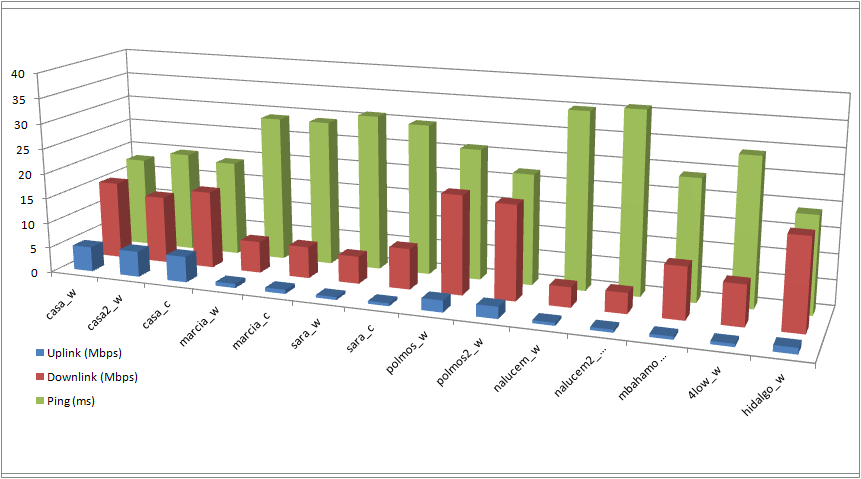
\includegraphics[scale=.45]{img/speed_graph}
		\caption{Speeds and Ping}
	\end{figure}
\end{frame}
\begin{frame}
	\frametitle{Results}
	\begin{block}{}
		\begin{itemize}
			\item The $\sim12ms$ ping were also not obtained, but the values are still within the acceptable range around the $\sim26ms$.
			\item The variation of the ratio between the measured and the bandwidth contracted is of 80\%, which is only 6\% less than spected.
		\end{itemize}
	\end{block}
\end{frame}


\begin{frame}
	\frametitle{Page Benchmark}
	\begin{figure}[h!]
		\centering
		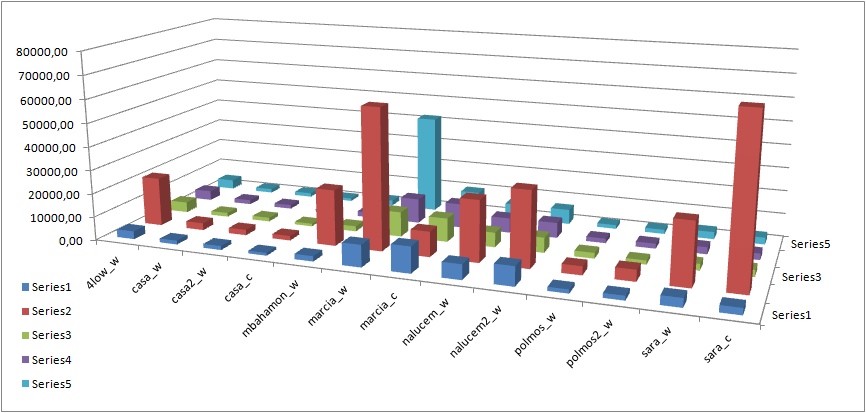
\includegraphics[scale=.45]{img/measures_page}
		\caption{Total Load Means in ms}
	\end{figure}
\end{frame}
\begin{frame}
	\frametitle{Results Overall}
	\begin{block}{}
		\begin{itemize}
			\item The average load for a problematic networks was over 9 (max 23) seconds. Normal load is between 1-7 (2) seconds. 
			\item The variation from minimun to maximum load was around 6 to 20 times.
		\end{itemize}
	\end{block}
\end{frame}

\begin{frame}
	\frametitle{Smokeping}
	\begin{figure} 
		\begin{subfigure}{\textwidth} 
			\centering 
			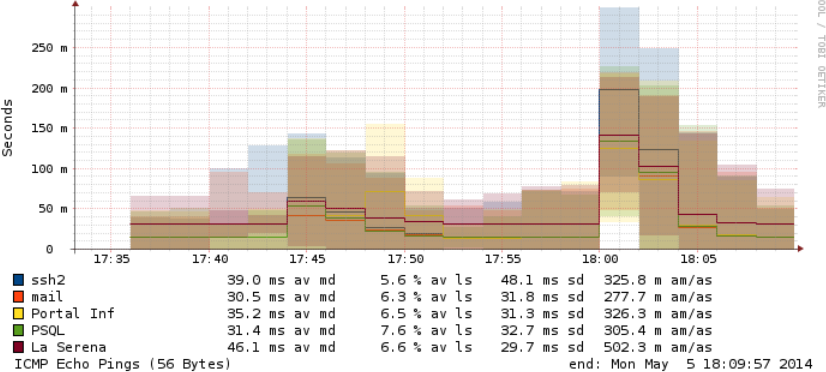
\includegraphics[width=0.6\textwidth]{img/smoke_nat_good} 
			\caption[Smokeping: Ping test to National servers with good performance]{Good performance Network} 
		\end{subfigure}% 
		\\ 
		\begin{subfigure}{\textwidth} 
			\centering 
			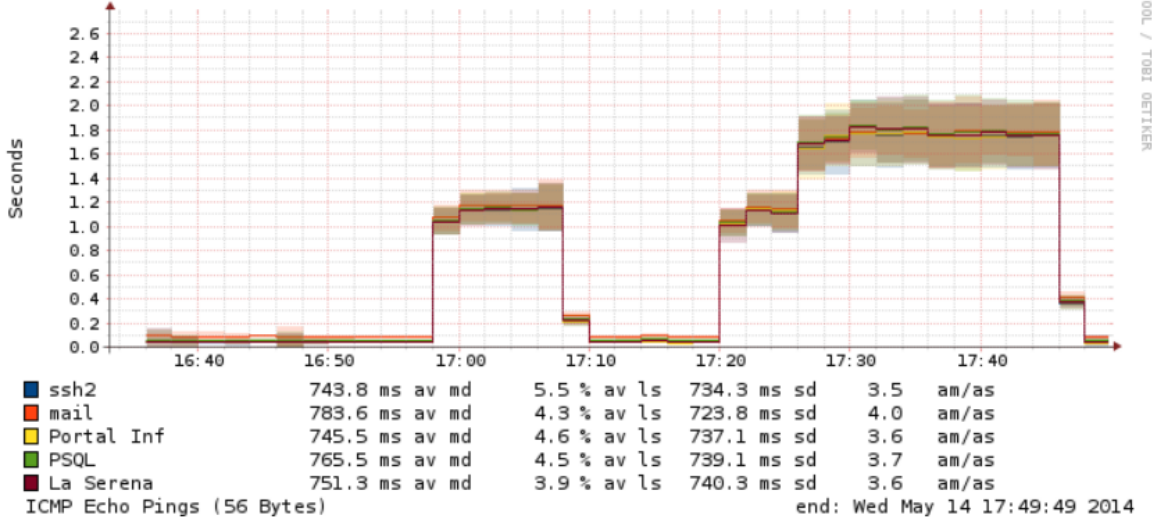
\includegraphics[width=0.6\textwidth]{img/smoke_nat_bad} 
			\caption[Smokeping: Ping test to National servers with bad performance]{Bad performance Network} 
		\end{subfigure} 
		\caption{Ping test to National servers} 
	\end{figure} 
\end{frame}


\begin{frame}
	\frametitle{Smokeping}
	\begin{figure}[h!]
		\centering 
		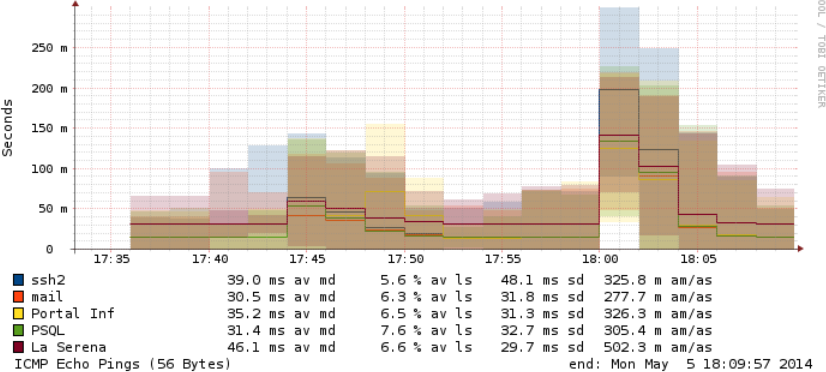
\includegraphics[scale=.35]{img/smoke_nat_good} 
		\caption[Smokeping: Ping test to National servers with good performance]{Good performance Network} 
	\end{figure}% 
\end{frame}
\begin{frame}
	\frametitle{Smokeping}
	\begin{figure}[h!]
			\centering 
			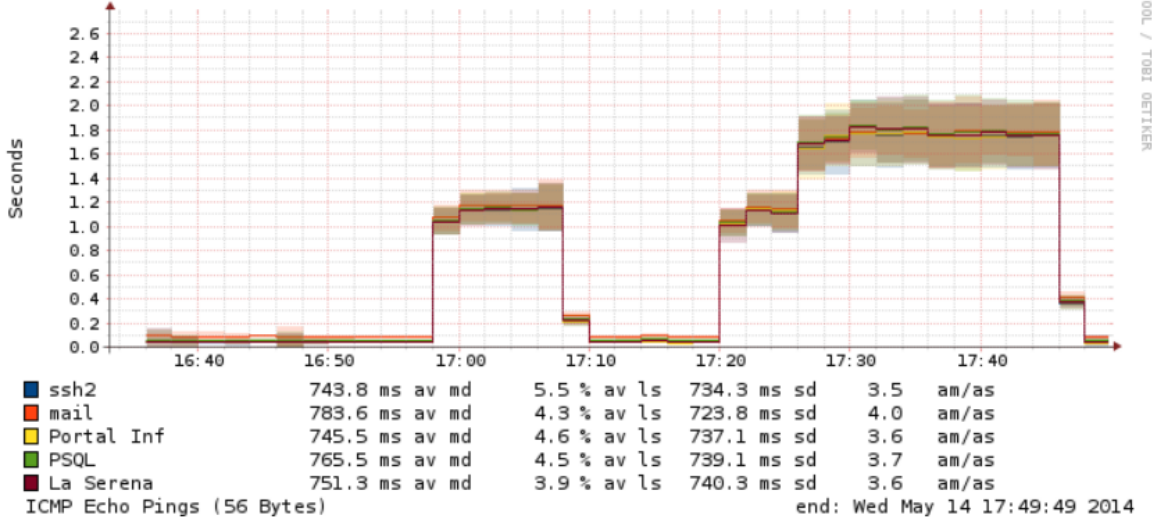
\includegraphics[scale=.35]{img/smoke_nat_bad} 
			\caption[Smokeping: Ping test to National servers with bad performance]{Bad performance Network} 
	\end{figure} 
\end{frame}


\begin{frame}
	\frametitle{Smokeping}
	\begin{figure} 
		\begin{subfigure}{\textwidth} 
			\centering 
			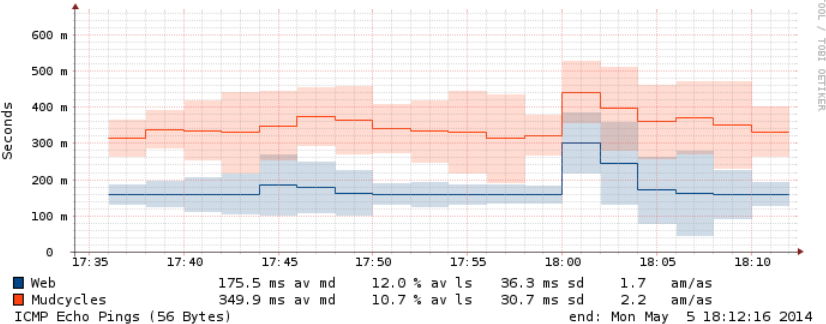
\includegraphics[width=0.6\textwidth]{img/smoke_int_good}
			\caption[Smokeping: Ping test to International Servers with good performance]{Good performance network}
		\end{subfigure}% 
		\\ 
		\begin{subfigure}{\textwidth} 
			\centering 
			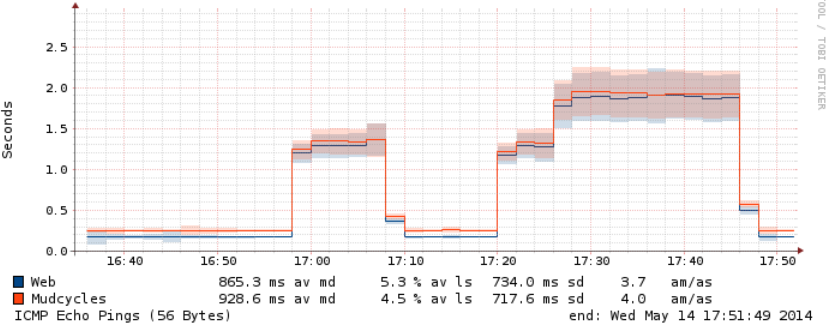
\includegraphics[width=0.6\textwidth]{img/smoke_int_bad}
			\caption[Smokeping: Ping test to International servers with bad performance]{Bad performance network}
		\end{subfigure}
		\caption[Smokeping: Ping test to International servers]{Ping test to International servers}
	\end{figure} 
\end{frame}


\begin{frame}
	\frametitle{Smokeping}
	\begin{figure}[h!]
		\centering 
			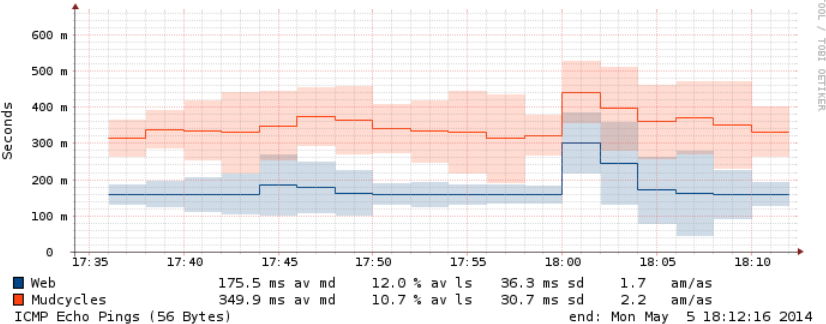
\includegraphics[scale=0.35]{img/smoke_int_good}
			\caption[Smokeping: Ping test to International Servers with good performance]{Good performance network}
	\end{figure}% 
\end{frame}
\begin{frame}
	\frametitle{Smokeping}
	\begin{figure}[h!] 
		\centering 
		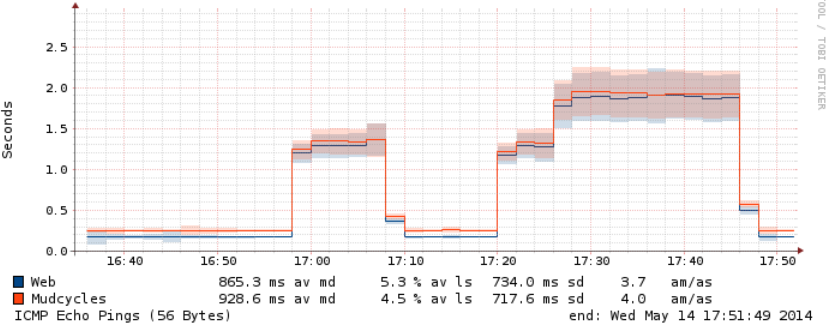
\includegraphics[scale=.35]{img/smoke_int_bad}
		\caption[Smokeping: Ping test to International servers with bad performance]{Bad performance network}
	\end{figure}
\end{frame}



\begin{frame}
	\frametitle{Smokeping}
	\begin{figure} 
		\begin{subfigure}{\textwidth} 
			\centering 
			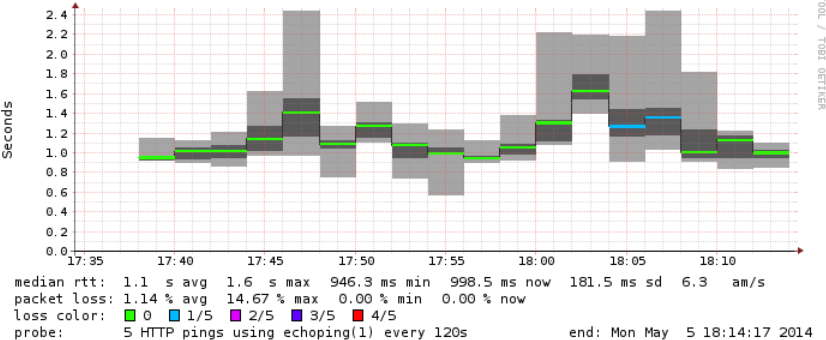
\includegraphics[width=0.6\textwidth]{img/smoke_inf_good}
			\caption[Smokeping: Web requests with good performance]{Good performance network}
		\end{subfigure}% 
		\\ 
		\begin{subfigure}{\textwidth} 
			\centering 
			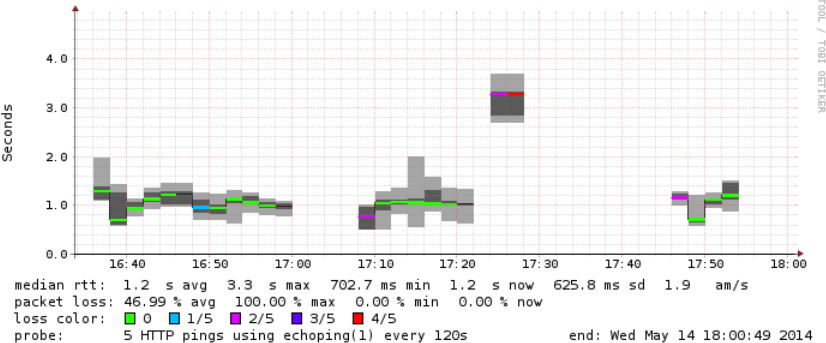
\includegraphics[width=0.6\textwidth]{img/smoke_inf_bad}
			\caption[Smokeping: Web requests with bad performance]{Bad performance network}
		\end{subfigure}
		\caption[Smokeping: Web requests to National servers]{Web requests to National servers}

	\end{figure} 
\end{frame}


\begin{frame}
	\frametitle{Smokeping}
	\begin{figure}[h!]
		\centering 
			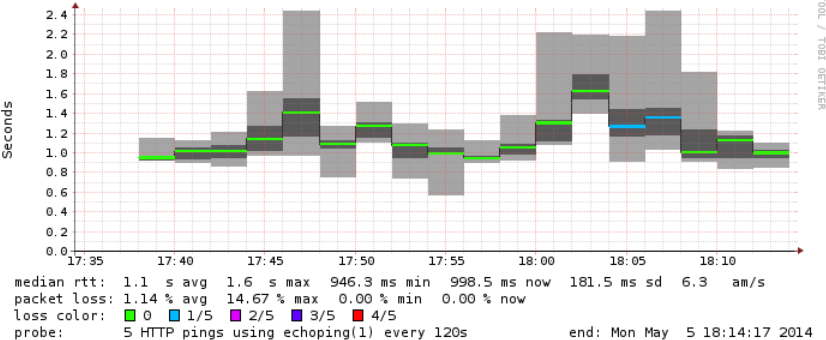
\includegraphics[scale=0.35]{img/smoke_inf_good}
			\caption[Smokeping: Web requests with good performance]{Good performance network}
	\end{figure}% 
\end{frame}
\begin{frame}
	\frametitle{Smokeping}
	\begin{figure}[h!]
			\centering 
			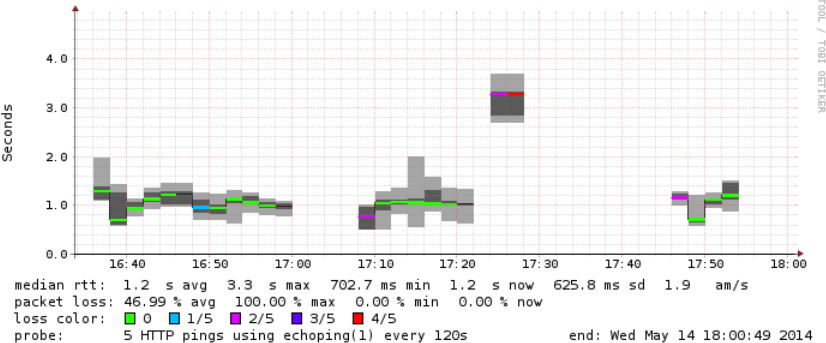
\includegraphics[scale=0.35]{img/smoke_inf_bad}
			\caption[Smokeping: Web requests with bad performance]{Bad performance network}
	\end{figure} 
\end{frame}
\begin{frame}
	\frametitle{Results Overall}
	\begin{block}{}
		\begin{itemize}
			\item The range for latency in a problematic network can be from 250ms to about 2 seconds.
			\item Lost related to problematic network can be over 70\% with 3 seconds to load and can reach to fully lost of communication.
		\end{itemize}
	\end{block}
\end{frame}


%%%%%%%%%%%%%%%% 10 Minutos %%%%%%%%%%%%%%%%%%%%%%
\section{Conclusions \& Discussion}
\begin{frame}
	\frametitle{Conclusions \tiny{[1/5]}}
	\begin{block}{}
	\begin{enumerate}
		\item \textit{A low latency network is wanted in order to exchange messages between a server and a client}.
	\end{enumerate}
\end{block}
\end{frame}
\begin{frame}
	\frametitle{Conclusions \tiny{[2/5]}}
	\begin{block}{}
	\begin{enumerate}
			\setcounter{enumi}{1}
		\item \textit{Having 12 times the latency when the network overload is not normal and as mentioned by Jim Gettys several times, the culprit is Bufferbloat}.
	\end{enumerate}
\end{block}
\end{frame}
\begin{frame}
	\frametitle{Conclusions \tiny{[3/5]}}
	\begin{block}{}
	\begin{enumerate}
			\setcounter{enumi}{2}
		\item \textit{Thanks to the various tests it was possible to demonstrate the presence and feel the effects of Bufferbloat in some networks}.
	\end{enumerate}
\end{block}
\end{frame}
\begin{frame}
	\frametitle{Conclusions \tiny{[4/5]}}
	\begin{block}{}
	\begin{enumerate}
			\setcounter{enumi}{3}
		\item \textit{With the advance in communications (evolution of real-time or on-demand apps.), the effects of phenomenons like Bufferbloat are more easily to feel and detect}.
	\end{enumerate}
\end{block}
\end{frame}
\begin{frame}
	\frametitle{Conclusions \tiny{[5/5]}}
	\begin{block}{}
	\begin{enumerate}
			\setcounter{enumi}{4}
		\item \textit{The larger the buffer size, the longer it takes for a packet to go through it, not adding any value in the packet transfer and only adding additional latency}.
	\end{enumerate}
\end{block}
\end{frame}

\begin{frame}
	\begin{block}{To keep in mind}
	\begin{itemize}
		\item Low Bandwidth $\rightarrow$ Bufferbloat?
		\item Low Latency or High Bandwidth?
		\item Why 12 times Lacenty??!!!!
		\item Benefits of bigger Buffers
	\end{itemize}
\end{block}
\end{frame}
%%%%%%%%%%%%%%%%%%%%%%%%%%%%%%%%%%%%

\begin{frame}
	\begin{block}{}
		\centering
		\textbf{Questions \& Comments}
	\end{block}
\end{frame}

\begin{frame}
	\begin{figure}[h!]
		\centering
		
\includegraphics[scale=.5]{img/listen}
	\end{figure}
\end{frame}

%%%%%%%%%%%%%%%%%%%%%%%%%%%%%%%%%%%%%%%%%%%%%%%%%%
\end{document}


